As mentioned in Section 3.4, there is currently a lack of existing tools that
provide a unified interface designed to inspect decomposed monolithic
architectures. Most available tools generate output files, such as JSON,
primarily intended for machine-to-machine communication rather than human
interpretation. As humans, our natural inclination is to comprehend information
visually, and visual representations allow us to understand better and grasp
the differences between decompositions. Visual representations can convey
complex concepts more effectively than textual representations, which require a
comprehensive understanding of the underlying structure. This notion aligns
with the widely famous saying, "A picture is worth a thousand words",
highlighting the power of visual representations in conveying information.
Therefore, developing an application that offers a visual representation of
decomposed monolithic architectures can significantly enhance the ability of
humans to comprehend and analyse the decomposition process.

\Cref{fig:comparison_page} provides a visual representation of three different
decompositions. Among these decompositions, two consist of clusters of
microservices generated through the decomposition of the same project.
Consequently, a connection exists between the modules within these two
decompositions, indicating the relationship between the corresponding
microservices. On the other hand, the third decomposition does not exhibit any
connection or relationship with the other two decompositions. This visual
representation helps users differentiate between the decompositions and
perceive the interconnection of modules within related decompositions while
highlighting the third decomposition's independent nature.

\begin{figure*}[!htb]
  \caption{Comparison Page} \label{fig:comparison_page}
  \centering
  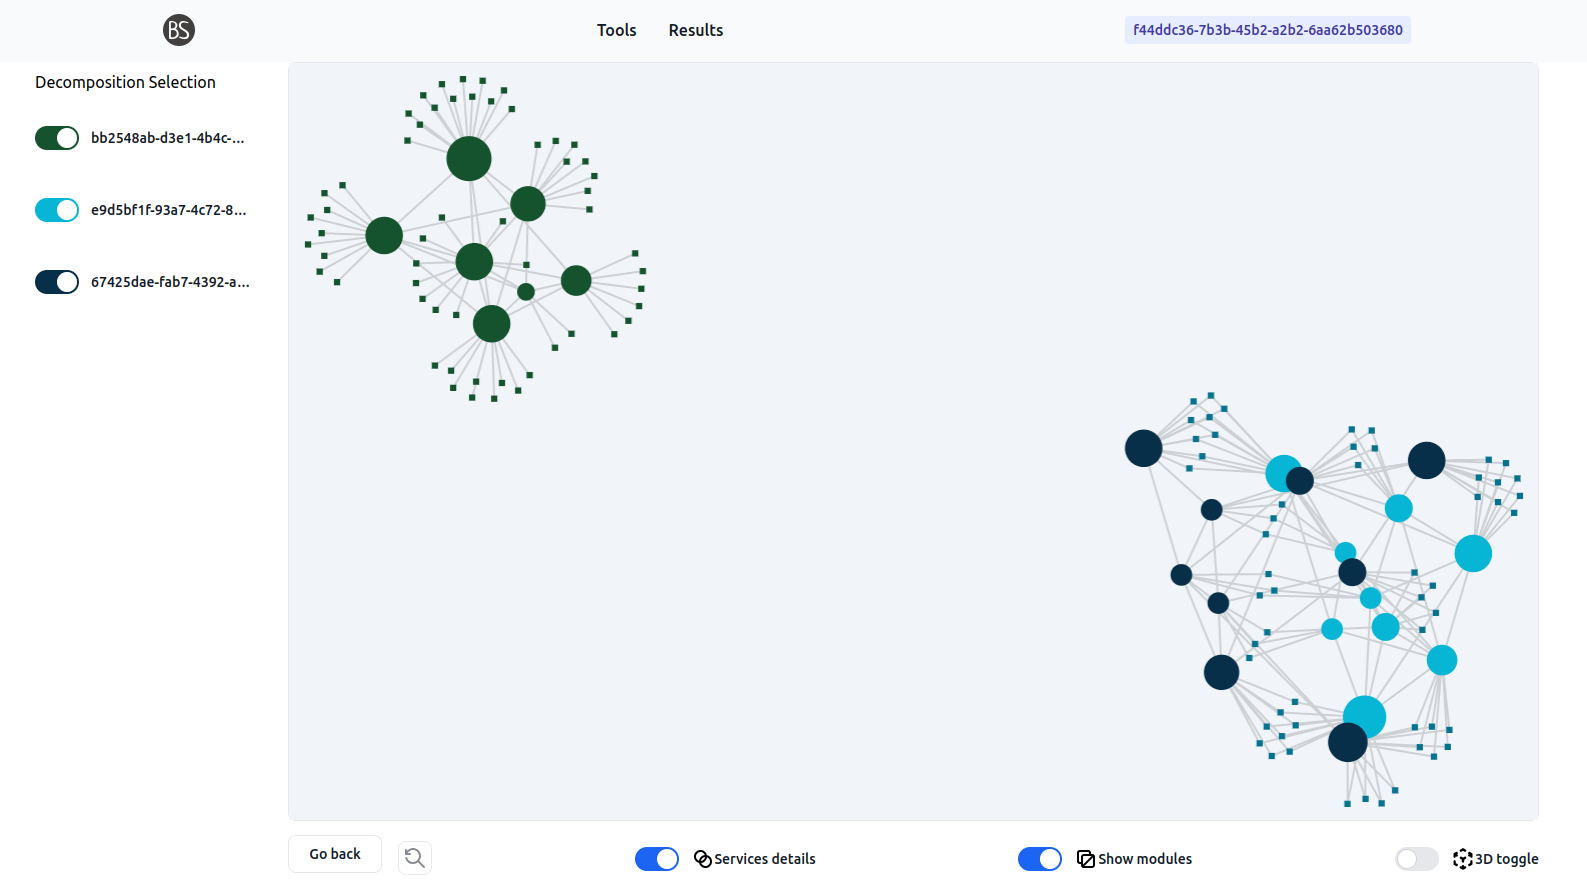
\includegraphics[width=\textwidth]{compare}
\end{figure*}

TODO: Alterar secção para quando o resumo da sec 3 estiver pronto.
